\chapter{Kalibrering}
\label{cha:kalibrering}

For at kunne oversætte mellem udstyrets kanalnummer og en given energi skulle der foretages en
kalibrering. Til dette formål blev der benyttet en kilde, der bestod af tre $\alpha$-kilder:
\ce{^{241}Am}, \ce{^{239}Pu} og \ce{^{244}Cm}.

Da forstærkningen er indstillet forskelligt i de enkelte strips og sektorer, er det nødvendigt at
kalibrere dem enkeltvisn. Linierne er skarpt adskilte og kalibreringen kan udføres ved at fitte
lineært til de pågældende centroid værdier.

Det skulle dog vise sig at være mere vanskeligt end først antaget, da detektoren havde et inativt
område, der blot bremsede partiklen uden at registrere energien. Dødlaget havde en tykkelse
$\Delta x$ på et par mikrometer, hvilket er illustreret på \cref{fig:deadLayer}.

Dødlaget har den effekt, at partikler, der rammer længere ude på detektoren, vil miste mere energi
end dem, der rammer de inderste strips, da de skal igennem en større vejlængde i dødlaget.

De relevante størrelser er den målte energi $E_{0}$, energien før dødlaget $E$ og vinklen $\phi$ mellem
partiklens hastighed og detektorens normal. Ud fra nogle enkelte geometriske betragtninger kan et
udtryk for $E$ opskrives
\begin{equation}
  \label{eq:deadE}
  E = E_{0} + \d{E}{x} \frac{\Delta x}{\cos \phi}  .
\end{equation}
Det sidste led er energitabet i dødlaget, som afhænger af materialets stoppeevne $\d{E}{x}$. Denne
antages at være konstant gennem dødlaget.

Det skal bemærkes, at dette er en approksimation, da producenten har oplyst, at dødlaget består både
af aluminium og silicium. Disse grundstoffer er hhv. nummer 13 og 14 i det periodiske system, så er
deres stoppeevne er stort set ens, og dødlaget approksimeres derfor til et enkelt lag silicium.
\begin{figure}[h]
  \centering
  \includegraphics[width=7cm]{DeadLayer}
  \caption{Skematisk tegning af S3 dektoren med et dødlag.}
  \label{fig:deadLayer}
\end{figure}

\section{Estimering af dødlagets tykkelse}
\label{sec:dodlag}

For at kunne bestemme tykkelsen af dødlaget er det nødvendigt at kende energien ved forskellige
vinkler, men som tidligere nævnt er forstærkningen indstillet forskelligt i ringene.

Løsningen på dette er at udvælge en radial sektor. Hver gang denne sektor bliver ramt, findes den
tilsvarende cirkulære strip. Kriteriet for dette er, at kanalnumrerne stemmer overens inden for en
vis tolerance. Dermed er det muligt at bestemme spektret for de enkelte cirkulære strips udtrykt i
kanalnummeret for den radiale sektor og derfor er der ingen forstærkning at tage højde for i
spektrene.

I alle disse spektre bestemmes centroidværdien af \Pu toppen.  Centroidværdien normaliseres til
kanalnummeret i strip 1 og plottes som funktion af $1/{\cos \phi}$. Ud over dette er
\cref{eq:deadE} også plottet for forskellige tykkelser. Disse er normaliseret til det teoretiske
udtryk for strip 1. Stoppeevnen er taget fra \cite{Ziegler}.

Det er ikke muligt at lave et fit til data med $\Delta x$ som en fri parameter, så tykkelsen af
dødlaget er vurderet ud fra de teoretiske kurver, som er plottet på \cref{fig:dead}. Data er
konsistent med en tykkelse på hhv. \SI{3.3(5)}{\um} og \SI{4.2(5)}{\um} for detektor 4 og 3. En
tilsvarende analyse er foretaget med S3 detektorerne roteret 180\degree. Her er resultatet, at
dødlaget var væsentlig mindre blot \SI{0.6(1)}{\um}. 

\begin{figure}[h]
  \centering
  \subbottom[Detektor 3]{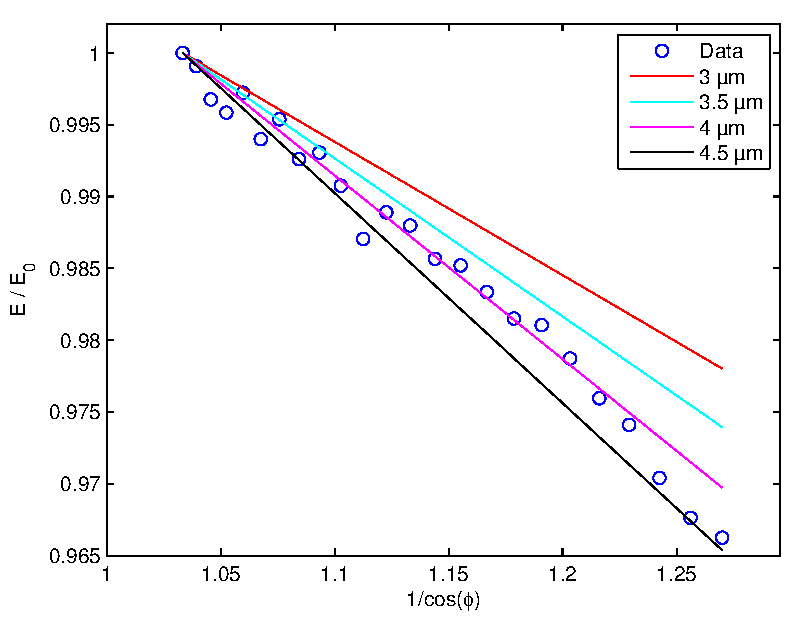
\includegraphics[width=0.47\columnwidth]{DeadLayerThin}}%
  \hfill
  \subbottom[Detektor 4]{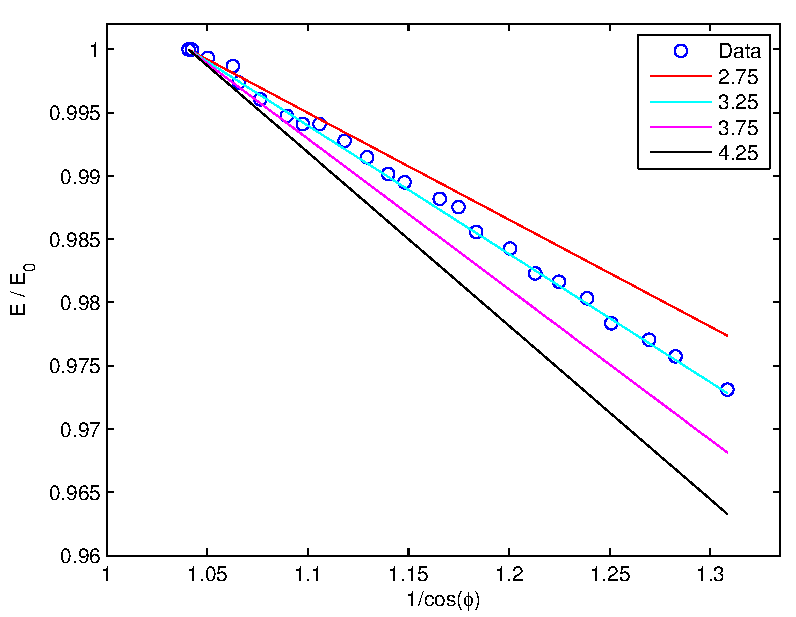
\includegraphics[width=0.47\columnwidth]{DeadLayerThick}}%
  \caption{De normaliserede energier som funktion af $1/{\cos\phi}$. Kurverne angiver det teoretiske
    udtryk givet i \cref{eq:deadE} og er plottet for forskellige tykkelser.}
  \label{fig:dead}
\end{figure}

\vspace{-5mm}
\section{Kalibreringsalgoritmen}
\label{sec:kalalgo}

Når tykkelsen er kendt, kan den målte energi $E_{0}$ bestemmes. Dermed kan vores detektorer
kalibreres. Under databehandlingen er det nødvendigt at bestemme energitabet for hver enkelt
hændelse, da energitabet afhænger af både indgangsenergien og partikeltypen.

For energier, hvor stoppeevnen er stor, vil det give anledning til fejl, hvis energitabet anses som
konstant hele vejen igennem materialet. Det samlede tab skal derfor udregnes ved integration og
i stedet benyttes middelrækkevidden for en partikel i et givent materiale. Ækvivalent til
\cref{eq:deadE} kan den samlede rækkevidde skrives som
\begin{equation}
  \label{eq:deadR}
  R(E) = R(E_{0}) + \frac{\Delta x}{\cos \phi} .
\end{equation}

Rækkeviden som funktion af energien er også tabuleret i \cite{Ziegler}, så for en given hændelse
blev $R(E_{0})$ bestemt ved lineær interpolation mellem de to nærmeste tabulerede værdier. Til dette
adderes tykkelsen af dødlaget, hvor der blev taget højde for vinklen. Den samme tabel blev også
benyttet den modsatte vej, hvor energien blev bestemt ud fra den samlede rækkevidde. Der blev igen
benyttet lineær interpolation.

Denne algoritme er anvendt til at lave \cref{fig:kalib-spec}, der viser det kalibrerede spektrum i
hhv. den inderste og yderste ring i detektor 3. 

\section{Resultater}
\label{sec:kalib-resultater}

I dette kapitel er der fremlagt data, der indikerer, at S3 detektorerne har et dødlag. På baggrund
af denne observation er der fremlagt en metode til at estimere tykkelsen af dødlagene. Med denne
metode blev det etableret, at dødlaget på bagsiden af detektorerne var 6-7 gange mindre end
forsidens og data i resten af rapporten vil være med detektorerne roteret 180\degree. Desuden er
der også præsenteret en kalibreringsalgoritme, der korrigerer for dødlaget. At algoritmen virker
efter hensigten vil blive verificeret i næste afsnit.

\begin{figure}[hb]
  \centering
  \vspace{-0.2cm}
  \subbottom[Inderste ring.]{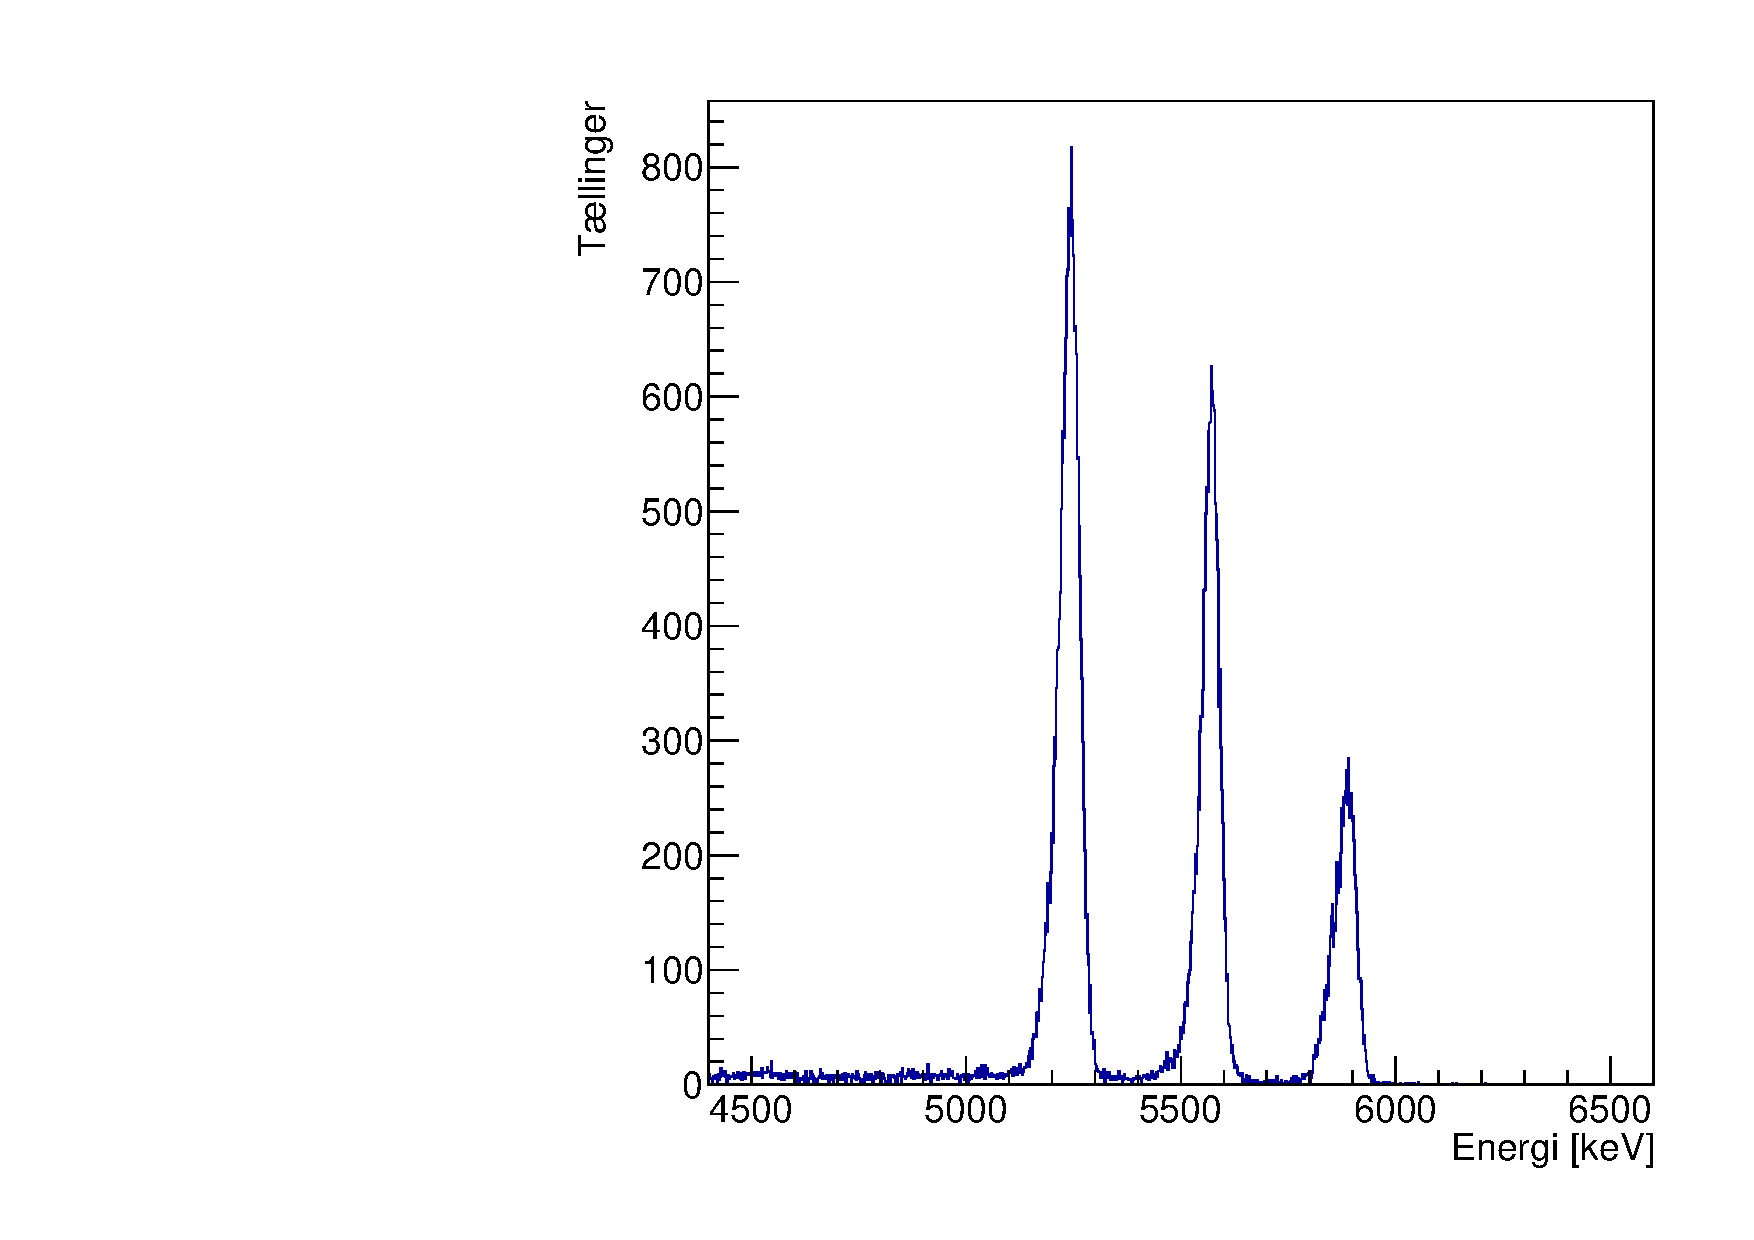
\includegraphics[width=0.4\columnwidth]{kalib-spec-inner}}%
  \hfill
  \subbottom[Yderste ring.]{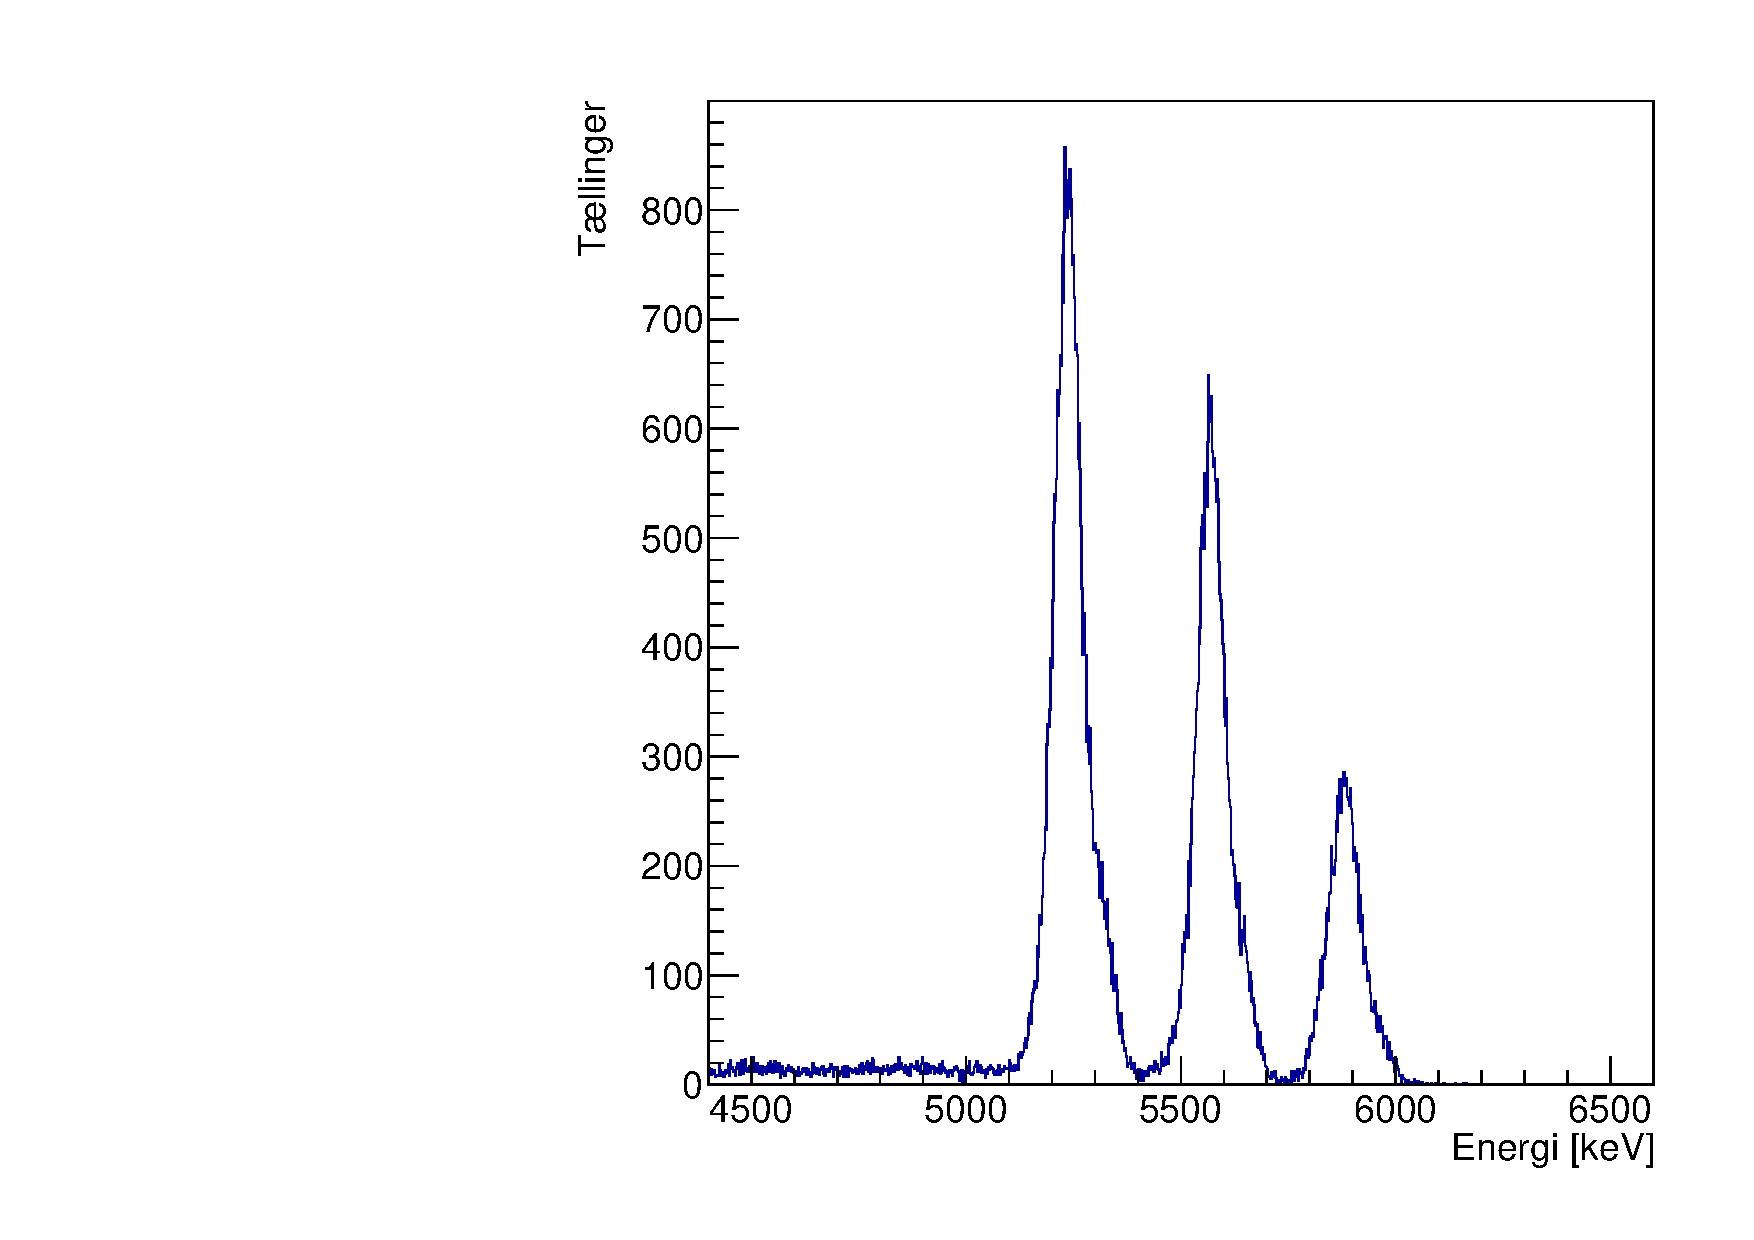
\includegraphics[width=0.4\columnwidth]{kalib-spec-outer}}%
  \caption{Energispektrum for henfaldskilden for detektor 3 med forsiden vendt mod kilden. Her er
    antaget, at dødlaget er \SI{4.2}{\um}.}
  \label{fig:kalib-spec}
  \vspace{-4cm}
\end{figure}









